\newpage

\section*{Anhang}
  \addcontentsline{toc}
    {section}
    {Anhang}



\subsection*{Elektronischer Anhang}\label{elect-anhang}
\addcontentsline{toc}
{subsection}
{Elektronischer Anhang}

Diese Dokumentation wurde zusammen mit einem elektronischen Anhang in Form einer ZIP-Datei abgegeben. Darin befinden sich der Simulator Programmiercode inklusive dessen Ergebnisse und die erstellten CAD Dateien.

\newpage
\subfile{parts/x-projektplanung}
\newpage

%%%%%%%%%%%%%%%%%% Aufgabenstellung

TOOD MAYBE SWITCH WITH NEW ONE FROM THIS SEMESTER?
\subsection{Originale Aufgabenstellung}\label{aufgabenstellung}

Nachfolgend ist die originale Aufgabenstellung angehängt.

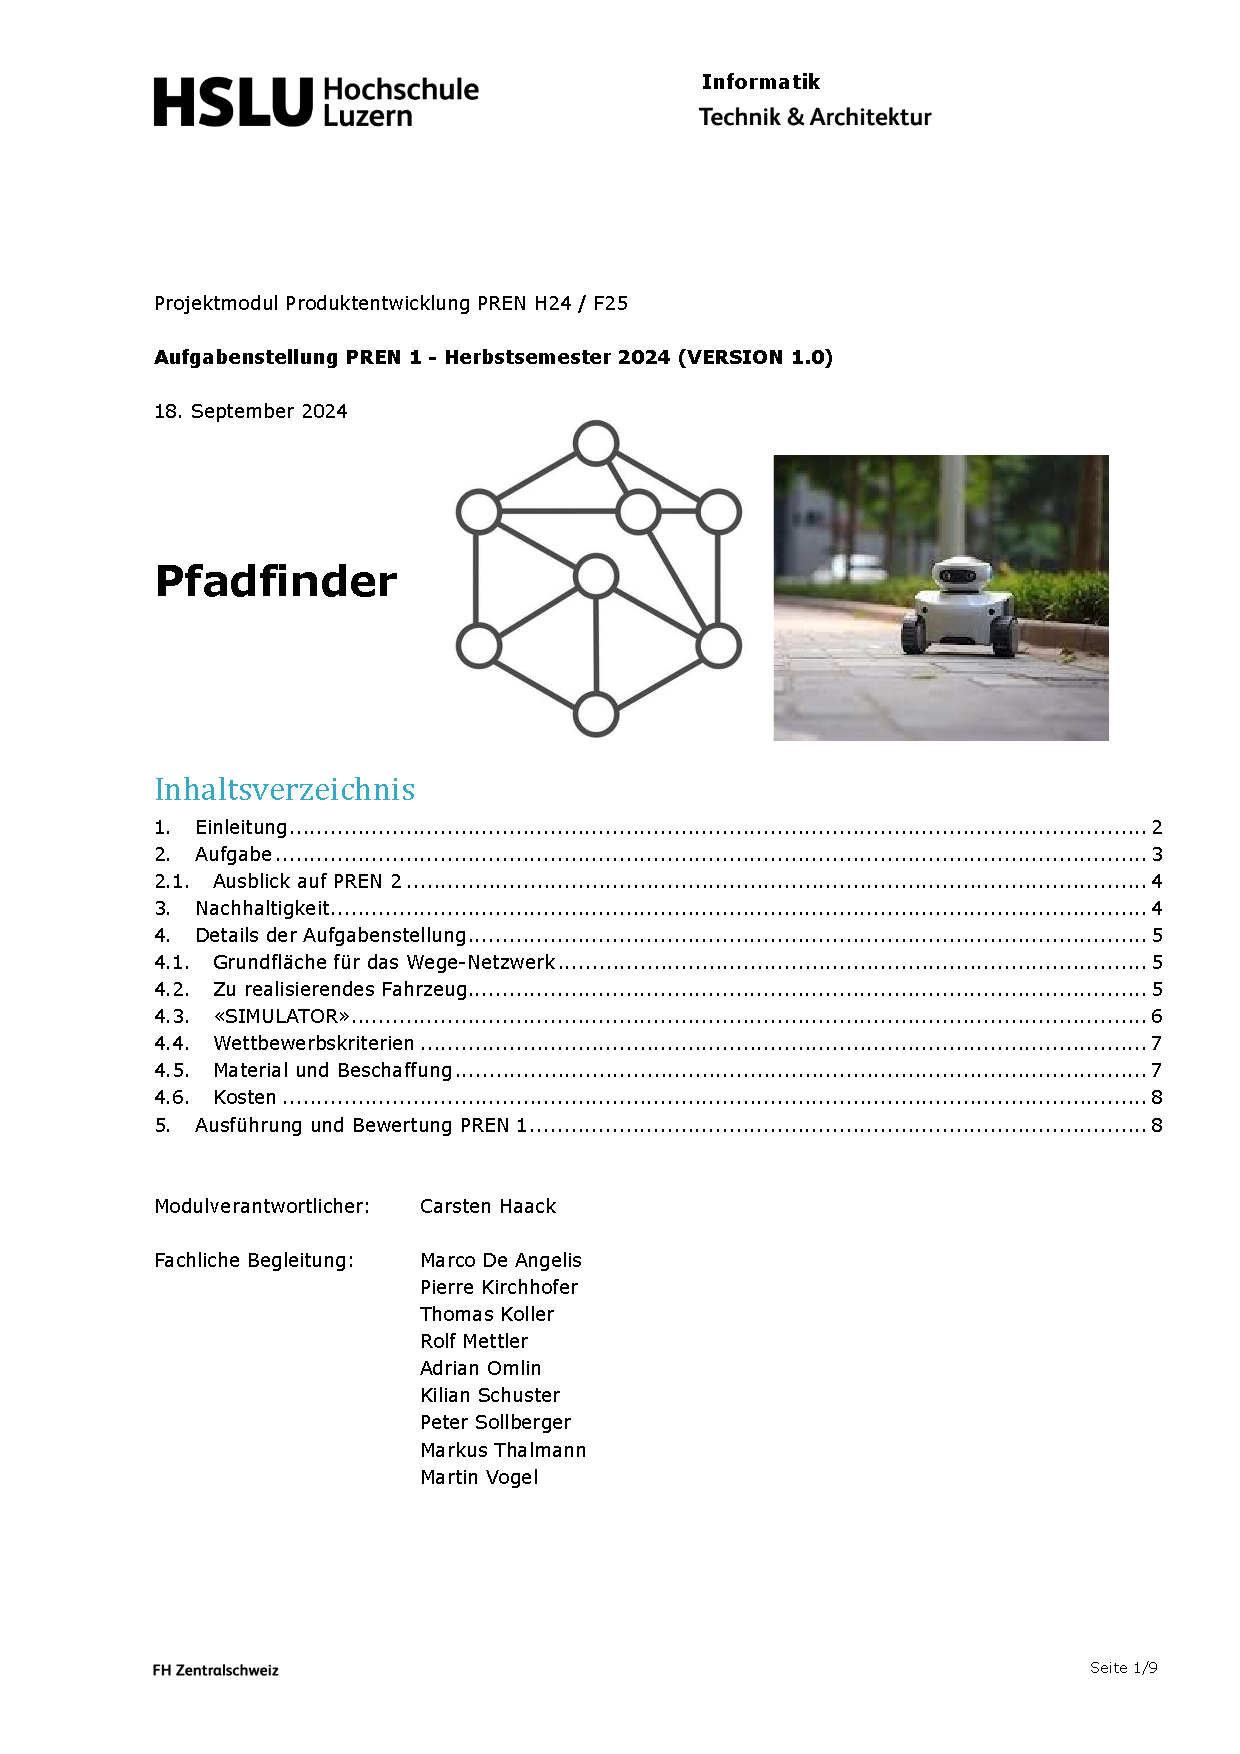
\includepdf[pages=-]{assets/projektmanagement/AufgabenstellungPREN1HS24.pdf}

%%%%%%%%%%%%%%% Anforderungsliste %%%%%%%%%%%%%%%%%%%%%%%%%

\subsection*{Anforderungsliste}\label{anforderungliste}
  \addcontentsline{toc}
    {subsection}
    {Anforderungsliste}
Die  Anforderungsliste ist ersichtlich in Tabellen \ref{table:anforderungsliste_page1} und \ref{table:anforderungsliste_page2}.

\begin{table}[H]
\centering
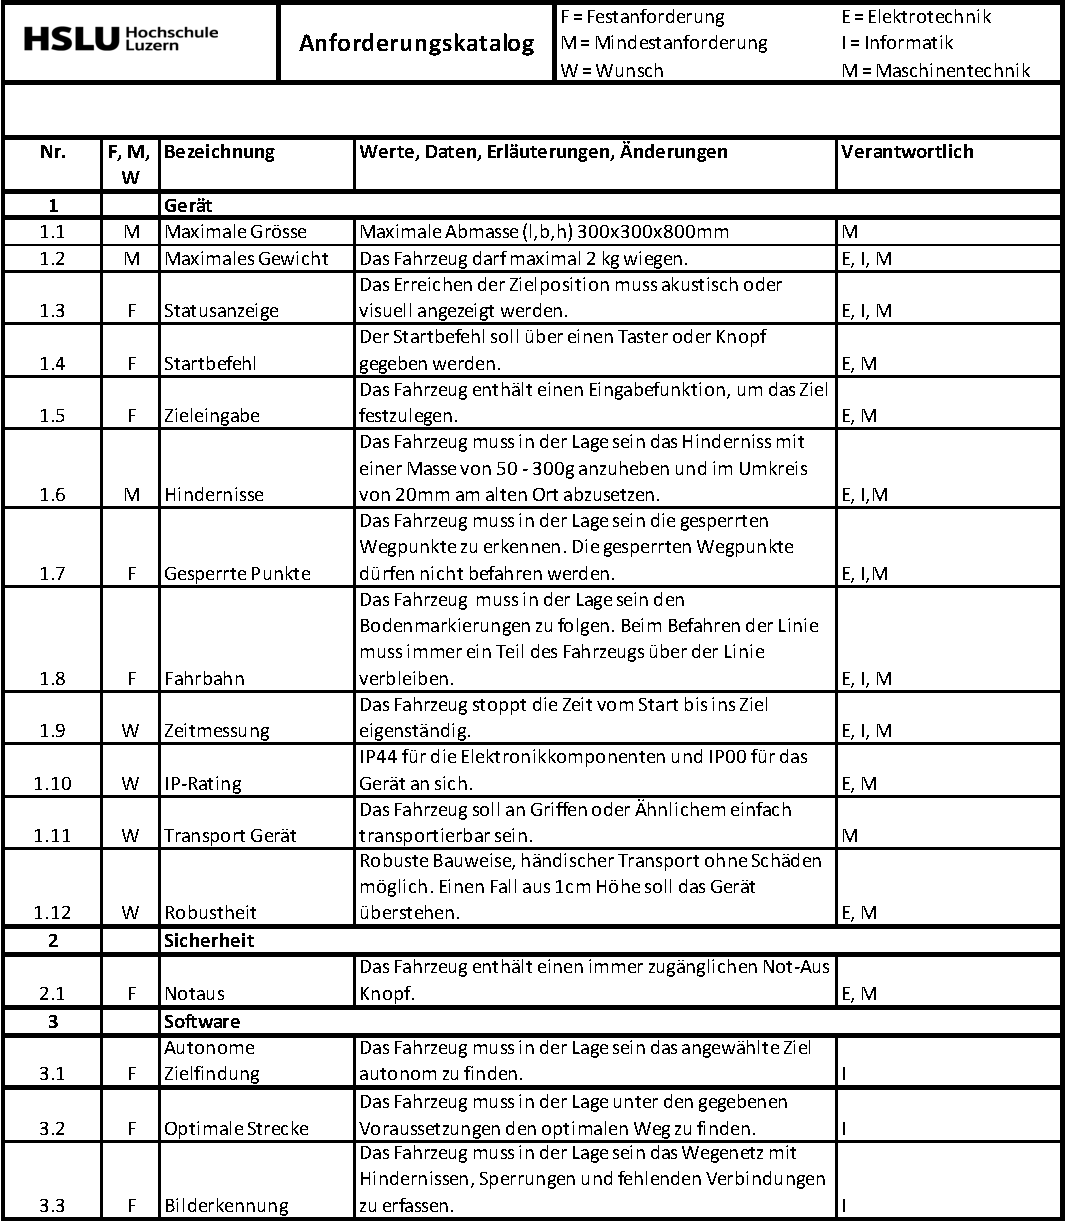
\includegraphics[width=\textwidth]{assets/projektmanagement/Anforderungsliste_V1.01_page1.pdf}
\caption{Anforderungsliste Teil 1}
\label{table:anforderungsliste_page1}
\end{table}
\newpage

\begin{table}[H]
\centering
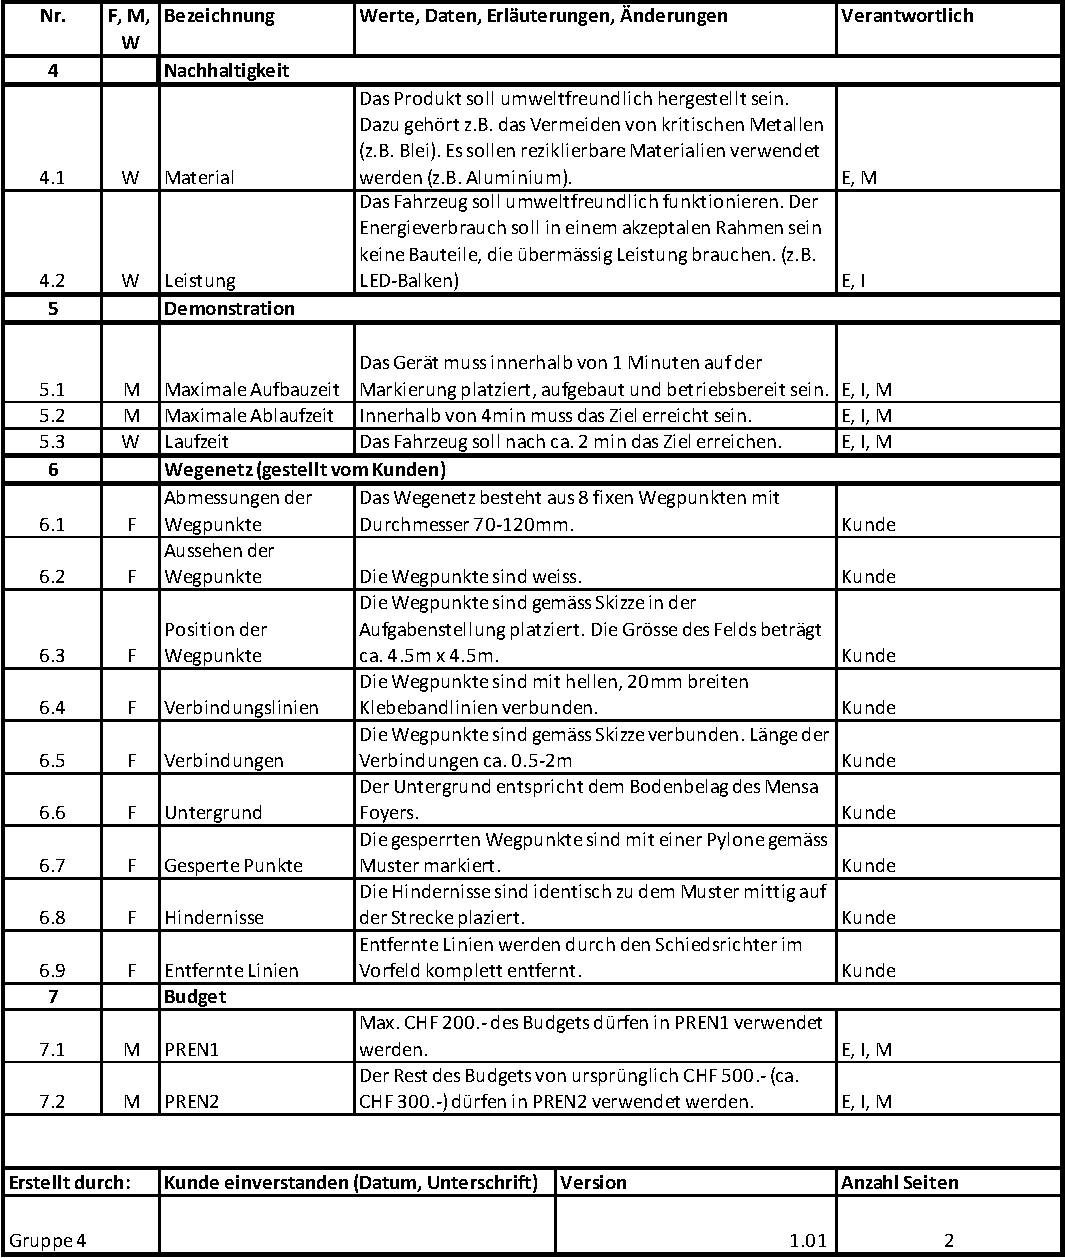
\includegraphics[width=\textwidth]{assets/projektmanagement/Anforderungsliste_V1.01_page2.pdf}
\caption{Anforderungsliste Teil 2}
\label{table:anforderungsliste_page2}
\end{table}
\newpage
